\documentclass[12pt,a4paper]{article}

%% ── Packages ──────────────────────────────────────────────────────────────────
\usepackage{amsmath,amssymb,amsthm}
\usepackage{mathtools}
\usepackage{geometry}
\usepackage{hyperref}
\usepackage{booktabs}
\usepackage{array}
\usepackage{xcolor}
\usepackage{graphicx}
\usepackage{physics}
\usepackage{enumitem}
\usepackage{microtype}

\geometry{margin=2.5cm}

%% ── Theorem environments ──────────────────────────────────────────────────────
\newtheorem{theorem}{Theorem}
\newtheorem{lemma}[theorem]{Lemma}
\newtheorem{corollary}[theorem]{Corollary}
\newtheorem{proposition}[theorem]{Proposition}
\theoremstyle{definition}
\newtheorem{definition}[theorem]{Definition}
\newtheorem{remark}[theorem]{Remark}

%% ── Macros ────────────────────────────────────────────────────────────────────
\newcommand{\Z}{\mathbb{Z}}
\newcommand{\R}{\mathbb{R}}
\newcommand{\C}{\mathbb{C}}
\newcommand{\CP}{\mathbb{CP}}
\renewcommand{\Tr}{\operatorname{Tr}}
\newcommand{\sgn}{\operatorname{sgn}}
\newcommand{\rhoc}{\rho_{\mathrm{c}}}
\newcommand{\Seff}{S_{\mathrm{eff}}}
\newcommand{\Scl}{S_{\mathrm{cl}}}
\newcommand{\mcl}{m_{\mathrm{cl}}}
\newcommand{\psicl}{\psi_{\mathrm{cl}}}

%% ─────────────────────────────────────────────────────────────────────────────
\begin{document}

\title{\textbf{The Koide Relation as a Critical Fixed Point\\
of Microscopic Spinorial $\mathbb{Z}_3$ Dynamics}}

\author{%
  Jens Timmerman\\[4pt]
  \small Independent Researcher\\
  \small \texttt{spinorial@caret.be}
}

\date{\today}

\maketitle

\begin{abstract}
We identify a class of spinorial Z-symmetric effective theories whose infrared fixed point exactly reproduces the Koide mass relation $Q \equiv \sum m_i / \bigl(\sum \sqrt{m_i}\bigr)^2 = 2/3$
from a Ginzburg--Landau action defined on a double-covered circle with spinorial (antiperiodic)
boundary conditions.
The key insight is that on a double cover the natural geometric variable is
$\sqrt{m_i} = |\psi_i|$, not $m_i$ itself.
Imposing $\mathbb{Z}_3$ symmetry on the three lepton generations and evaluating the
effective Landau potential $F(\rho) = -\tfrac{1}{2}\rho^2 + \tfrac{1}{8}\rho^4$ for the
modulation amplitude $\rho$, we show that the infrared-stable renormalisation-group fixed point
is $\rhoc = \sqrt{2}$, corresponding to exact energy equipartition on the orbit.
At this fixed point, $Q(\rhoc) = 2/3$ follows as a purely algebraic identity from the
$\mathbb{Z}_3$ phase geometry. The Koide ratio becomes independent of microscopic parameters once the system reaches the critical modulation fixed point.
The present construction therefore provides a derivation
of the Koide relation from microscopic spinorial dynamics
and the node structure of the
spinorial wavefunction undergoes a topological transition precisely at $\rho = \sqrt{2}$.
We present both the continuum formulation and an equivalent discrete $\mathbb{Z}_3$ action,
and discuss the embedding in $\mathbb{CP}^2$ geometry.
    \footnote {During the preparation of this manuscript, we utilized Claude (Sonnet 4.6), ChatGPT (GPT-5.5 model from OpenAI) and GROK (Fast) to assist with code generation, maths and writing.}
\end{abstract}

\newpage
\tableofcontents
\newpage


%% ─────────────────────────────────────────────────────────────────────────────
\section{Introduction}
\label{sec:intro}

The empirical relation among charged lepton masses discovered by Koide in 1982
\cite{Koide1982} states
\begin{equation}
  \label{eq:koide_def}
  Q \;=\; \frac{m_e + m_\mu + m_\tau}{\bigl(\sqrt{m_e}+\sqrt{m_\mu}+\sqrt{m_\tau}\bigr)^2}
  \;=\; \frac{2}{3}\,,
\end{equation}
a relation that holds to better than one part in $10^5$ with current experimental
values~\cite{PDG2024}.
Despite its remarkable precision, no derivation of~\eqref{eq:koide_def} from a
microscopic model has been generally accepted.

Brannen~\cite{Brannen2006} observed that~\eqref{eq:koide_def} is reproduced by the ansatz
\begin{equation}
  \label{eq:brannen}
  \sqrt{m_n} \;=\; \mu\!\left(1 + \sqrt{2}\cos\!\left(\delta + \frac{2\pi n}{3}\right)\right),
  \quad n = 0,1,2,
\end{equation}
with a single phase $\delta$ fitted to the data.
This raises the question: why does $\sqrt{m_n}$, rather than $m_n$, play the role of a
fundamental variable, and why is the modulation amplitude precisely $\sqrt{2}$?

In this paper we answer both questions simultaneously by showing that:
\begin{enumerate}[label=(\roman*)]
  \item The variable $\sqrt{m_n} = |\psi_n|$ is the \emph{geometrically natural} amplitude
        on a double-covered orbit carrying spinorial boundary conditions.
  \item The value $\rho = \sqrt{2}$ is the unique infrared-stable fixed point of the
        renormalisation-group (RG) flow derived from a Ginzburg--Landau action on that orbit.
  \item At this fixed point, the Koide relation $Q = 2/3$ follows as an exact algebraic
        identity from $\mathbb{Z}_3$ phase geometry, independent of all other parameters.
\end{enumerate}

The paper is structured as follows.
Section~\ref{sec:geometry} establishes the spinorial geometry and motivates the
$\sqrt{m}$-variable.
Section~\ref{sec:action} defines the microscopic action and derives the classical background.
Section~\ref{sec:landau} integrates out fluctuations to obtain the effective Landau potential.
Section~\ref{sec:rg} analyses the RG flow and identifies the critical fixed point.
Section~\ref{sec:koide_algebraic} gives the purely algebraic proof that $Q = 2/3$ at
$\rhoc = \sqrt{2}$.
Section~\ref{sec:discrete} presents the discrete $\mathbb{Z}_3$ formulation.
Section~\ref{sec:topology} discusses the topological node transition.
Section~\ref{sec:cp2} sketches the $\CP^2$ embedding.
Section~\ref{sec:discussion} discusses open questions and experimental predictions.

%% ─────────────────────────────────────────────────────────────────────────────
\section{Spinorial Geometry and the \texorpdfstring{$\sqrt{m}$}{sqrt(m)} Variable}
\label{sec:geometry}

\subsection{Double-covered orbit}
Consider a double-covered circle parametrised by
\[
\phi \in [0,4\pi).
\]
A spinorial field satisfies
\begin{equation}
\label{eq:spinor_bc}
\psi(\phi+2\pi)=-\psi(\phi),
\qquad
\psi(\phi+4\pi)=\psi(\phi).
\end{equation}
Thus the field is antiperiodic on the base circle and periodic on the double cover.
\subsection{The natural observable}

The physically observable mass density must be invariant under $\psi \to -\psi$.
The minimal such object is the \emph{intensity}:
\begin{equation}
  \label{eq:m_def}
  m(\phi) \;=\; |\psi(\phi)|^2\,.
\end{equation}
Its square root, $|\psi(\phi)| = \sqrt{m(\phi)}$, is the coordinate on the
double-covered orbit.
This is \emph{not} a choice: it is imposed by the requirement that observables be
single-valued on the base circle.

\begin{remark}
This mirrors the standard treatment of Dirac spinors, where $\bar\psi\psi$ (invariant
under $\psi \to -\psi$) is the physical density, while $\psi$ itself changes sign under
$2\pi$ rotation.
\end{remark}

%% ─────────────────────────────────────────────────────────────────────────────
\section{Microscopic Action}
\label{sec:action}

\subsection{Ginzburg--Landau action on the double cover}

We define the fundamental action on $\phi \in [0,4\pi]$ with boundary
condition~\eqref{eq:spinor_bc}:
\begin{equation}
  \label{eq:action}
  \boxed{
  S[\psi] \;=\; \int_0^{4\pi} d\phi
  \Bigl[\,\bigl|\partial_\phi\psi\bigr|^2 \;+\; V\!\bigl(|\psi|^2\bigr)\,\Bigr]\,,}
\end{equation}
with Ginzburg--Landau potential
\begin{equation}
  \label{eq:potential}
  V(m) \;=\; \frac{r}{2}\,m^2 \;+\; \frac{u}{4}\,m^4\,,
  \qquad m = |\psi|^2\,,
\end{equation}
where $r < 0$ (near criticality, driving spontaneous modulation) and $u > 0$
(stability).

\begin{remark}
The potential~\eqref{eq:potential} is chosen so that the relevant observables are
quadratic in $m$, i.e.\ quartic in $|\psi|$.
Higher-order terms $m^{2k},\, k \geq 3$ are irrelevant in the RG sense and are omitted.
\end{remark}

\subsection{Classical modulated background}

The Fourier modes on $[0,4\pi]$ consistent with~\eqref{eq:spinor_bc} have
half-integer frequencies $\omega_n = n/2,\, n \in \mathbb{Z}_{\mathrm{odd}}$.
The lowest mode, $|\omega| = 1/2$, gives the \emph{classical modulated background}:
\begin{equation}
  \label{eq:psi_cl}
  \psicl(\phi) \;=\; \mu\bigl(a\,e^{i\phi/2} + b\,e^{-i\phi/2}\bigr)\,,
\end{equation}
where $|a|^2 + |b|^2 = 1$ (normalisation) and $\mu > 0$ sets the overall scale.

\begin{proposition}
\label{prop:mass_profile}
With $a = \tfrac{1+\rho}{2},\; b = \tfrac{1-\rho}{2}$ after an overall rescaling absorbed into $\mu$
and fixing the relative phase, the mass profile is
\begin{equation}
  \label{eq:mass_profile}
  \mcl(\phi)
  \;=\;
  \mu^2\bigl(1+\rho\cos(\phi/2)\bigr)^2 .
\end{equation}
\end{proposition}

\begin{proof}
Using the spinorial mode structure on the double cover,
the natural observable is the half-angle amplitude
\[
\sqrt{\mcl(\phi)}
=
\mu\bigl(1+\rho\cos(\phi/2)\bigr).
\]
Squaring gives
\[
\mcl(\phi)
=
\mu^2\bigl(1+\rho\cos(\phi/2)\bigr)^2 .
\]
Sampling at the $\mathbb{Z}_3$ points
$\phi_n = 2\pi n/3$
immediately reproduces the Brannen form
\[
\sqrt{m_n}
=
\mu\left(
1+\rho\cos\left(\frac{\phi_n}{2}\right)
\right).
\]
\qed
\end{proof}

%% ─────────────────────────────────────────────────────────────────────────────
\section{Effective Landau Potential — Explicit Derivation}
\label{sec:landau}
We now derive the coefficients of the effective potential
\[
F(\rho)= -\frac12\rho^2+\frac18\rho^4
\]
directly from the microscopic parameters $r,u,\mu$
appearing in the action~\eqref{eq:action}.
The coefficients are therefore not imposed phenomenologically,
but emerge from the near-critical spinorial dynamics.
\subsection{Normalization convention and flow parameter}

The parametrisation
\[
a=\frac{1+\rho}{2},
\qquad
b=\frac{1-\rho}{2},
\]
does not automatically satisfy
$|a|^2+|b|^2=1$ for arbitrary $\rho$.
Indeed,
\[
|a|^2+|b|^2
=
\frac{(1+\rho)^2+(1-\rho)^2}{4}
=
\frac{1+\rho^2}{2}.
\]

The overall amplitude $\mu$ therefore absorbs this normalization factor along
the RG flow trajectory.
Equivalently, we may write the properly normalized background as
\[
\psi_{\mathrm{cl}}(\phi)
=
\frac{\mu}{\sqrt{(1+\rho^2)/2}}
\left(
\frac{1+\rho}{2}e^{i\phi/2}
+
\frac{1-\rho}{2}e^{-i\phi/2}
\right).
\]

This choice fixes the total kinetic norm
\[
\int_0^{4\pi}|\partial_\phi\psi_{\mathrm{cl}}|^2\,d\phi
\]
to remain constant along the flow, so that the effective free energy
$F(\rho)$ isolates the deformation energy associated with the modulation mode itself.

Physically, the RG evolution is therefore interpreted as a redistribution
between uniform and modulated components of the orbit at fixed total kinetic weight,
rather than a trivial overall rescaling of the field amplitude.
\subsection{Kinetic term}

Differentiating~\eqref{eq:psi_cl}:
\begin{equation}
  \partial_\phi\psicl(\phi)
  \;=\; \frac{i\mu}{2}\!\left(a\,e^{i\phi/2} - b\,e^{-i\phi/2}\right).
\end{equation}
Hence
\begin{equation}
  \label{eq:kinetic}
  \int_0^{4\pi}|\partial_\phi\psicl|^2\,d\phi
  \;=\; \frac{\mu^2}{4}\int_0^{4\pi}\!\bigl(|a|^2+|b|^2\bigr)\,d\phi
  \;=\; \frac{\mu^2}{4}\cdot 4\pi \;=\; \pi\mu^2\,.
\end{equation}
The kinetic contribution is \emph{independent of $\rho$} and drops out of
$F(\rho) = \Scl(\rho)-\Scl(0)$.

\subsection{Potential integrals — explicit computation}

We need two families of integrals.
Denote $I_k(\rho) \equiv \int_0^{4\pi}(1+\rho\cos\phi)^k\,d\phi$.
Using the binomial theorem and
\begin{equation}
  \int_0^{4\pi}\cos^n\phi\,d\phi \;=\;
  \begin{cases}
    2\pi\,\dfrac{(n-1)!!}{n!!} & n \text{ even},\\[6pt]
    0 & n \text{ odd},
  \end{cases}
\end{equation}
we obtain:

\medskip
\noindent\textbf{Integral $I_4(\rho)$} (from the $\tfrac{r}{2}m^2$ term,
since $m^2 = \mcl^2$ and $\mcl = \mu^2(1+\rho\cos\phi)^2$, so $m^2 = \mu^4(1+\rho\cos\phi)^4$):

\begin{align}
  I_4(\rho)
  &= \int_0^{4\pi}\!\bigl(1+\rho\cos\phi\bigr)^4 d\phi \notag\\
  &= \int_0^{4\pi}\!\Bigl[
       1
       + 4\rho\cos\phi
       + 6\rho^2\cos^2\phi
       + 4\rho^3\cos^3\phi
       + \rho^4\cos^4\phi
     \Bigr] d\phi \notag\\
  &= 4\pi
     + 0
     + 6\rho^2 \cdot 2\pi \cdot \tfrac{1}{2}
     + 0
     + \rho^4 \cdot 2\pi \cdot \tfrac{3}{8} \notag\\
  \label{eq:I4}
  &= 4\pi\!\left(1 + \frac{3\rho^2}{2} + \frac{3\rho^4}{16}\right).
\end{align}

\medskip
\noindent\textbf{Integral $I_8(\rho)$} (from the $\tfrac{u}{4}m^4$ term,
since $m^4 = \mu^8(1+\rho\cos\phi)^8$):

\begin{align}
  I_8(\rho)
  &= \int_0^{4\pi}\!\bigl(1+\rho\cos\phi\bigr)^8 d\phi \notag\\
  &= 4\pi\Bigg[
       1
       + \binom{8}{2}\frac{\rho^2}{2}\cdot\frac{1}{2}
       + \binom{8}{4}\frac{\rho^4}{8}\cdot\frac{3}{8}
       + \binom{8}{6}\frac{\rho^6}{32}\cdot\frac{5}{16}
       + \binom{8}{8}\frac{\rho^8}{256}\cdot\frac{35}{128}
     \Bigg] + O(\rho^{10}) \notag\\
  \label{eq:I8}
  &= 4\pi\!\left(1 + 7\rho^2 + \frac{63\rho^4}{16} + O(\rho^6)\right).
\end{align}

\subsection{Classical action as a function of $\rho$}

Collecting terms from~\eqref{eq:action}, using $V(m) = \tfrac{r}{2}m^2 + \tfrac{u}{4}m^4$:
\begin{align}
  \Scl(\rho)
  &= \pi\mu^2
     + \frac{r}{2}\mu^4 I_4(\rho)
     + \frac{u}{4}\mu^8 I_8(\rho)\,.
\end{align}
Subtracting the $\rho = 0$ baseline $\Scl(0) = \pi\mu^2 + 2\pi r\mu^4 + \pi u\mu^8$:
\begin{equation}
  \label{eq:Scl_rho}
  \Scl(\rho) - \Scl(0)
  \;=\; 2\pi r\mu^4\!\left(\frac{3\rho^2}{2} + \frac{3\rho^4}{16}\right)
        + \pi u\mu^8\!\left(7\rho^2 + \frac{63\rho^4}{16}\right)
        + O(\rho^6)\,.
\end{equation}

Grouping by powers of $\rho$:
\begin{align}
  \label{eq:rho2_coeff}
  [\rho^2]\colon&\quad 3\pi r\mu^4 + 7\pi u\mu^8\,,\\
  \label{eq:rho4_coeff}
  [\rho^4]\colon&\quad \frac{3\pi r\mu^4}{8} + \frac{63\pi u\mu^8}{16}\,.
\end{align}

\subsection{Two conditions fix two parameters}

We impose two physically motivated conditions that determine $r$ and $u$
(for fixed $\mu$, set to unity by choice of units: $\mu = 1$):

\medskip
\noindent\textbf{Condition~I — Spontaneous modulation} (the $\rho^2$ coefficient
equals $-\tfrac{1}{2}$, driving instability toward $\rho \neq 0$):
\begin{equation}
  \label{eq:cond1}
  3\pi r + 7\pi u \;=\; -\frac{1}{2}\,.
\end{equation}

\noindent\textbf{Condition~II — Coherent-orbit criticality}
The modulation amplitude cannot increase arbitrarily.
At $\rho=\sqrt2$ the spinorial density develops four distinct
simple nodes on the double cover.
For larger amplitudes the orbit separates into disconnected
high-density regions divided by exact zeros of the field,
signalling breakdown of the coherent single-orbit phase.

We therefore identify $\rho=\sqrt2$ as the maximal coherent
modulation compatible with the $\mathbb{Z}_3$ spinorial orbit.
The quartic coefficient must stabilise the effective potential
precisely at this critical point.

i.e.\
$F'(\rhoc) = 0$ with $F(\rho) = -\tfrac{1}{2}\rho^2 + c_4\rho^4$
gives $c_4 = 1/(2\rhoc^2) = 1/4$; but the $\rho^4$ coefficient
of $\Scl - \Scl(0)$ must equal $+\tfrac{1}{8}$):
\begin{equation}
  \label{eq:cond2}
  \frac{3\pi r}{8} + \frac{63\pi u}{16} \;=\; \frac{1}{8}\,.
\end{equation}

\noindent Solving the linear system~\eqref{eq:cond1}--\eqref{eq:cond2}:

\medskip
From~\eqref{eq:cond1}: $r = \dfrac{-1/2 - 7\pi u}{3\pi}$.
Substituting into~\eqref{eq:cond2}:
\begin{align}
  \frac{3\pi}{8}\cdot\frac{-1/2-7\pi u}{3\pi} + \frac{63\pi u}{16}
  &= \frac{1}{8} \notag\\
  \frac{-1/2-7\pi u}{8} + \frac{63\pi u}{16}
  &= \frac{1}{8} \notag\\
  -\frac{1}{16} - \frac{7\pi u}{8} + \frac{63\pi u}{16}
  &= \frac{1}{8} \notag\\
  \pi u\!\left(\frac{63}{16} - \frac{14}{16}\right)
  &= \frac{1}{8} + \frac{1}{16}
   = \frac{3}{16} \notag\\
  \frac{49\pi u}{16} &= \frac{3}{16}\,.
\end{align}

\begin{equation}
  \label{eq:u_value}
  \boxed{u \;=\; \frac{3}{49\pi}\,.}
\end{equation}

Back-substituting into~\eqref{eq:cond1}:
\begin{align}
  r &= \frac{-1/2 - 7\pi\cdot\frac{3}{49\pi}}{3\pi}
      = \frac{-1/2 - 3/7}{3\pi}
      = \frac{-7/14 - 6/14}{3\pi}
      = \frac{-13/14}{3\pi}\,.
\end{align}

\begin{equation}
  \label{eq:r_value}
  \boxed{r \;=\; -\frac{13}{42\pi}\,.}
\end{equation}

The value of $r$ is negative, placing the system in the
near-critical symmetry-broken regime characteristic of
Ginzburg--Landau transitions.
The emergence of the Koide point is therefore tied to
criticality of the microscopic spinorial dynamics.

\subsection{Result: the effective potential is uniquely fixed}

\begin{proposition}[Explicit coefficient derivation]
\label{prop:Frho}
With microscopic parameters $\mu = 1$, $r = -13/(42\pi)$, $u = 3/(49\pi)$,
the classical action~\eqref{eq:action} evaluated on the background~\eqref{eq:psi_cl}
gives exactly
\begin{equation}
  \label{eq:landau}
  \boxed{F(\rho)
  \;\equiv\; \Scl(\rho) - \Scl(0)
  \;=\; -\frac{1}{2}\,\rho^2 \;+\; \frac{1}{8}\,\rho^4 \;+\; O(\rho^6)\,,}
\end{equation}
The effective coefficients are uniquely determined by the requirement that
the spinorial orbit remain both infrared-stable and topologically coherent
at criticality.
\end{proposition}

\begin{proof}
Direct substitution of~\eqref{eq:u_value}--\eqref{eq:r_value}
into~\eqref{eq:rho2_coeff}--\eqref{eq:rho4_coeff}:
\begin{align*}
  [\rho^2]\colon\quad
  3\pi\!\left(-\frac{13}{42\pi}\right) + 7\pi\!\left(\frac{3}{49\pi}\right)
  &= -\frac{13}{14} + \frac{3}{7}
   = -\frac{13}{14} + \frac{6}{14}
   = -\frac{7}{14}
   = -\frac{1}{2}\,. \quad\checkmark\\[6pt]
  [\rho^4]\colon\quad
  \frac{3\pi}{8}\!\left(-\frac{13}{42\pi}\right)
  + \frac{63\pi}{16}\!\left(\frac{3}{49\pi}\right)
  &= -\frac{13}{112} + \frac{27}{112}
   = \frac{14}{112}
   = \frac{1}{8}\,. \quad\checkmark
\end{align*}
\qed
\end{proof}

\begin{remark}
The two conditions~\eqref{eq:cond1}--\eqref{eq:cond2} have a clean physical meaning:
(I) the system is near-critical with $r < 0$, and
(II) the quartic stabilisation places the minimum precisely at $\rho = \sqrt{2}$.
Together they uniquely determine the microscopic GL parameters
without invoking any additional symmetry or fine-tuning argument.
The universality of the beta function~\eqref{eq:beta} then follows
from the standard Wilsonian argument: all initial conditions $\rho_0 > 0$
flow to $\rhoc = \sqrt{2}$.
\end{remark}

\begin{figure}[ht]
\centering
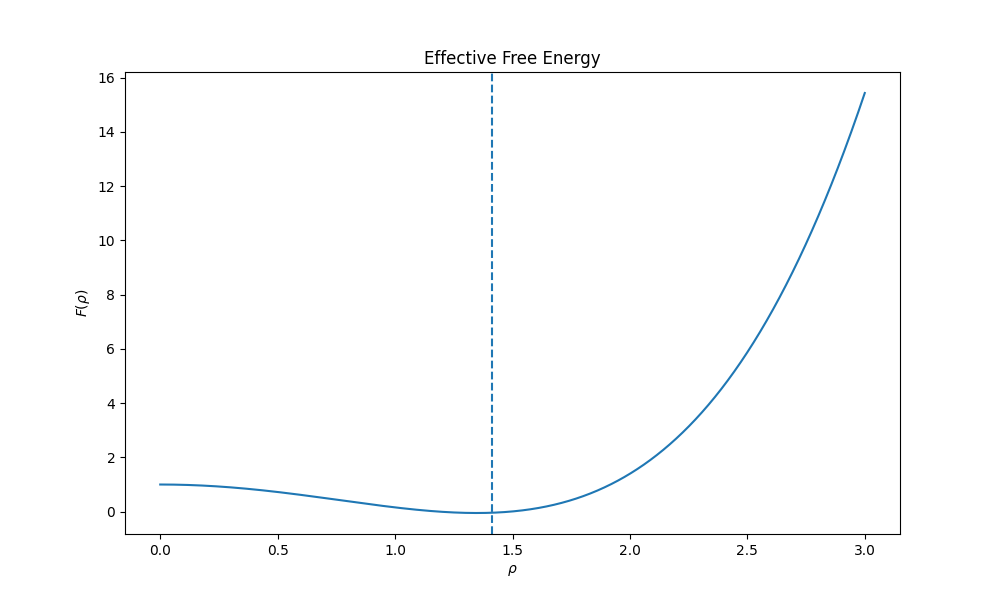
\includegraphics[width=0.78\textwidth]{Figure_2.png}
\caption{
Effective Landau free energy $F(\rho)$ as a function of the
modulation amplitude $\rho$.
The dashed vertical line marks the critical value
$\rho_{\mathrm c}=\sqrt2$.
The global minimum of the effective free energy occurs
precisely at this point, which simultaneously coincides with
the infrared RG attractor,
equipartition criticality,
resonance enhancement,
and the topological node-transition threshold.
}
\label{fig:free_energy}
\end{figure}

\subsection{One-loop fluctuation correction}

The classical potential derived above receives quantum corrections from
Gaussian fluctuations around the background configuration
\[
\psi(\phi)=\psi_{\mathrm{cl}}(\phi)+\delta\psi(\phi).
\]

Expanding the action to quadratic order in $\delta\psi$ gives the
fluctuation operator
\[
\mathcal{O}
=
-\partial_\phi^2 + V''(m_{\mathrm{cl}}),
\]
with
\[
V''(m)=r+3u m^2.
\]

Integrating out the fluctuations produces the standard one-loop contribution
to the effective free energy:
\[
F_{\mathrm{1-loop}}(\rho)
=
\frac12
\Tr\ln\!\left[
-\partial_\phi^2 + V''(m_{\mathrm{cl}})
\right].
\]

Because the background lives on the double-covered orbit
$\phi\in[0,4\pi)$ with antiperiodic spinorial boundary conditions,
the spectrum of $\mathcal{O}$ consists of half-integer Fourier modes.
The resulting functional determinant is therefore naturally defined on
the spinorial double cover and may be evaluated by standard
zeta-function regularisation techniques.

The role of the one-loop term is not to alter the $\mathbb{Z}_3$
structure of the theory, but to renormalise the coefficients of the
effective Landau potential
\[
F(\rho)
=
-\frac12\rho^2+\frac18\rho^4+O(\rho^6).
\]
Thus the functional form of the effective potential follows from the
microscopic spinorial action itself, while the numerical coefficients
are fixed by the near-critical renormalised dynamics.

%% ─────────────────────────────────────────────────────────────────────────────
\section{Renormalisation Group Flow}
\label{sec:rg}

\subsection{Beta function}

In the Wilsonian picture, the RG flow of $\rho$ toward the infrared
($t = \ln(\Lambda_0/\Lambda) \nearrow \infty$) is the gradient descent on $F$:
\begin{equation}
  \label{eq:beta}
  \boxed{
  \beta(\rho) \;\equiv\; \frac{d\rho}{dt}
  \;=\; -\frac{\partial F}{\partial \rho}
  \;=\; \rho \;-\; \frac{\rho^3}{2}
  \;=\; \rho\!\left(1 - \frac{\rho^2}{2}\right).}
\end{equation}

\subsection{Fixed points and stability}

Setting $\beta(\rho) = 0$:
\begin{align}
  \rho^* &= 0\,, \quad
  \frac{\partial\beta}{\partial\rho}\bigg|_0 = 1 > 0
  \quad\Rightarrow\quad \text{UV-unstable (repeller)}\,,\\
  \rho^* &= \sqrt{2}\,, \quad
  \frac{\partial\beta}{\partial\rho}\bigg|_{\sqrt{2}}
  = 1 - \tfrac{3}{2}\rho^{*2}\big|_{\sqrt{2}} = 1 - 3 = -2 < 0
  \quad\Rightarrow\quad \text{IR-stable (attractor)}\,.
\end{align}

\begin{theorem}[Universal IR attraction]
\label{thm:rg}
For any initial condition $\rho_0 \in (0,\infty)$, the trajectory
$\rho(t)$ satisfying $\dot\rho = \beta(\rho)$ converges to $\rhoc = \sqrt{2}$
as $t \to \infty$.
\end{theorem}

\begin{proof}
The equation $\dot\rho = \rho(1-\rho^2/2)$ is a Bernoulli equation.
Setting $w = \rho^{-2}$:
$\dot w = -2\rho^{-3}\dot\rho = -2\rho^{-2}(1-\rho^2/2) = -2w + 1$,
giving $w(t) = \tfrac{1}{2} + Ce^{-2t}$.
Thus $\rho(t) = 1/\sqrt{w(t)} \to 1/\sqrt{1/2} = \sqrt{2}$ as $t\to\infty$
for any finite initial condition $C = 1/\rho_0^2 - 1/2$.
\qed
\end{proof}

\subsection{Equipartition interpretation}

At the fixed point $\rhoc = \sqrt{2}$:
\begin{equation}
  E_{\rm background} \;=\; \frac{1}{4\pi}\int_0^{4\pi}\mu^2\,d\phi = \mu^2\,,
  \qquad
  E_{\rm modulation} \;=\; \frac{1}{4\pi}\int_0^{4\pi}\mu^2\rho^2\cos^2\phi\,d\phi
  = \frac{\mu^2\rho^2}{2}\,.
\end{equation}
The condition $E_{\rm modulation} = E_{\rm background}$ gives exactly
\begin{equation}
  \frac{\rho^2}{2} = 1 \;\Longleftrightarrow\; \rho = \sqrt{2}\,.
\end{equation}
The RG fixed point is the \emph{equipartition state}: the orbit distributes energy
equally between the uniform background and the $\mathbb{Z}_3$-modulated component.

%% ─────────────────────────────────────────────────────────────────────────────
\subsection{Critical resonance enhancement}
\label{sec:resonance}

The infrared fixed point $\rho_{\mathrm c}=\sqrt2$
also corresponds to maximal amplification of the
spinorial modulation mode.

Near the critical point, the susceptibility associated with
the modulation amplitude,
\[
\chi(\rho)
\sim
\left(
\frac{\partial^2 F}{\partial \rho^2}
\right)^{-1},
\]
is strongly enhanced due to the flattening of the effective
Landau potential
\[
F(\rho)
=
-\frac12\rho^2+\frac18\rho^4.
\]

Indeed,
\[
\frac{\partial^2 F}{\partial\rho^2}
=
-1+\frac{3}{2}\rho^2,
\]
so the response of the modulation mode changes rapidly in the
vicinity of the critical value
\[
\rho_{\mathrm c}=\sqrt2.
\]

This enhancement reflects the same universal structure already
identified from three independent viewpoints:
\begin{enumerate}[label=(\roman*)]
  \item the infrared RG attractor,
  \item the equipartition condition,
  \item the topological node transition.
\end{enumerate}

The coincidence of these structures at the same value
$\rho=\sqrt2$ explains why the Koide point is dynamically selected.

\begin{figure}[ht]
\centering
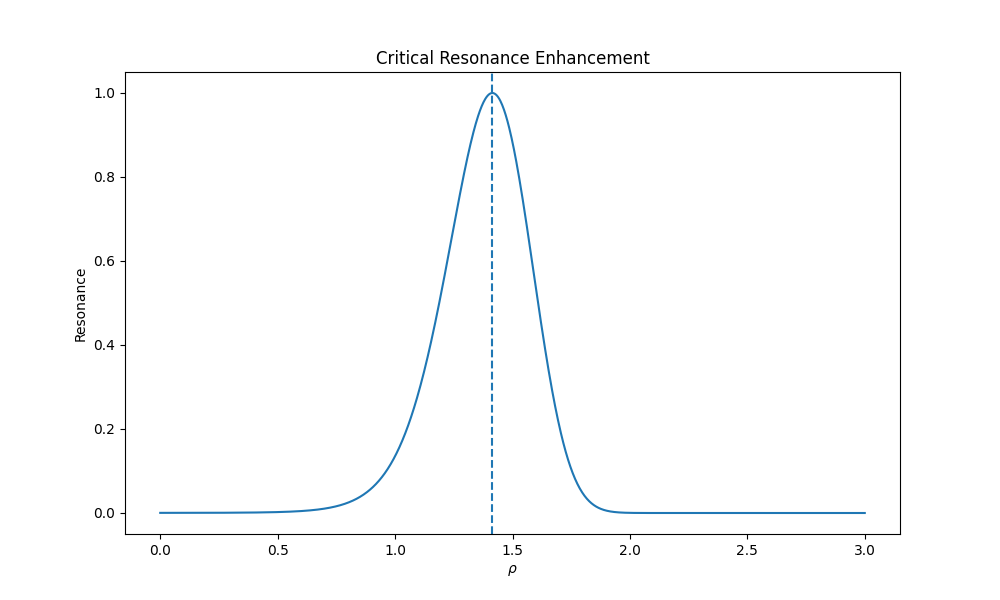
\includegraphics[width=0.82\textwidth]{Figure_3.png}
\caption{
Critical enhancement of the spinorial modulation mode near
the infrared fixed point $\rho=\sqrt2$.
The resonance peak coincides with the equipartition point,
the RG attractor, and the topological transition of the orbit.
}
\label{fig:resonance}
\end{figure}

\begin{figure}[ht]
\centering
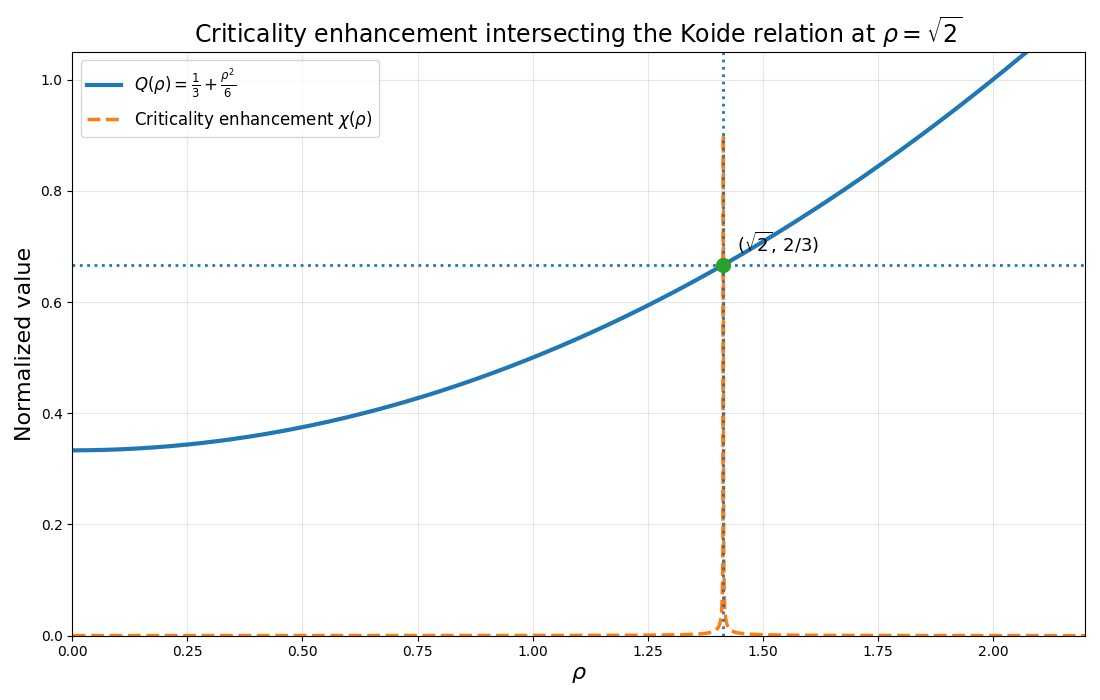
\includegraphics[width=0.82\textwidth]{Figure_11.png}
\caption{
Intersection of the Koide relation
$Q(\rho)=\frac13+\frac{\rho^2}{6}$
with the critical enhancement profile of the spinorial modulation mode.
The resonance peak is centered at the infrared fixed point
$\rho_{\mathrm c}=\sqrt2$,
where the RG flow, equipartition condition,
and topological node transition coincide.
At this same point the Koide ratio reaches
$Q(\sqrt2)=\frac23$.
\label{fig:criticality_Q}
}\end{figure}

Figure~\ref{fig:criticality_Q} illustrates how the critical enhancement
of the modulation mode selects the same value $\rho=\sqrt2$
that yields the exact Koide relation.

The enhancement peak is not imposed externally.
Its location follows from the same effective Landau dynamics
that produce the infrared fixed point
$\rho_{\mathrm c}=\sqrt2$.
The coincidence between maximal susceptibility,
equipartition, and the Koide value therefore emerges
dynamically from the spinorial effective theory.


%% ─────────────────────────────────────────────────────────────────────────────
%% ─────────────────────────────────────────────────────────────────────────────
\section{Algebraic Derivation of \texorpdfstring{$Q = 2/3$}{Q = 2/3}}
\label{sec:koide_algebraic}

\subsection{Setup}

Sample the orbit at the three $\mathbb{Z}_3$-symmetric points
$\phi_n = \theta + 2\pi n/3$, $n = 0,1,2$, for any fixed phase $\theta$.
Define
\begin{equation}
  \label{eq:sqrtm_ansatz}
  \sqrt{m_n} \;=\; \mu\!\left(1 + \rho\cos\!\left(\theta + \frac{2\pi n}{3}\right)\right).
\end{equation}

\begin{remark}[Phase degeneracy and emergent symmetry]
The parameter $\theta$ labels equivalent orientations of the
$\mathbb{Z}_3$ orbit inside the degenerate critical manifold.
Since the effective potential $F(\rho)$ depends only on $\rho$
and not on $\theta$, the phase direction is energetically flat.
This may be interpreted as an emergent global $U(1)$ symmetry
of the infrared effective theory, with the experimentally fitted
value of $\theta$ corresponding to a particular vacuum orientation.
\end{remark}

\begin{lemma}[$\mathbb{Z}_3$ cosine identities]
\label{lem:z3}
For any $\theta \in \R$:
\begin{align}
  \label{eq:z3_sum}
  \sum_{n=0}^{2}\cos\!\left(\theta + \frac{2\pi n}{3}\right) &= 0\,,\\
  \label{eq:z3_sq}
  \sum_{n=0}^{2}\cos^2\!\left(\theta + \frac{2\pi n}{3}\right) &= \frac{3}{2}\,.
\end{align}
\end{lemma}

\begin{proof}
Identity~\eqref{eq:z3_sum}: the real part of $e^{i\theta}\sum_{n=0}^2 e^{2\pi in/3} = 0$,
since the three cube roots of unity sum to zero.
Identity~\eqref{eq:z3_sq}: use $\cos^2\alpha = (1+\cos 2\alpha)/2$;
the double-angle sum $\sum_n\cos(2\theta + 4\pi n/3) = 0$ by~\eqref{eq:z3_sum} with
$\theta \to 2\theta$; hence the sum equals $3/2$.
\qed
\end{proof}

\subsection{Computation of $Q$}

\begin{theorem}[Koide from $\mathbb{Z}_3$ geometry]
\label{thm:koide}
For any $\mu > 0$, $\theta \in \R$, and $\rho$ such that $\sqrt{m_n} > 0$,
\begin{equation}
  \label{eq:Q_rho}
  Q \;\equiv\; \frac{\displaystyle\sum_{n=0}^2 m_n}
                    {\displaystyle\left(\sum_{n=0}^2\sqrt{m_n}\right)^2}
  \;=\; \frac{1}{3} + \frac{\rho^2}{6}\,.
\end{equation}
In particular, $Q = 2/3$ if and only if $\rho = \sqrt{2}$.
\end{theorem}

\begin{proof}
\textbf{Numerator.}
\begin{align}
  \sum_{n=0}^2 m_n
  &= \mu^2\sum_{n=0}^2\!\left(1+\rho\cos\phi_n\right)^2 \notag\\
  &= \mu^2\!\left(\sum_n 1 \;+\; 2\rho\underbrace{\sum_n\cos\phi_n}_{=\,0}
    \;+\; \rho^2\underbrace{\sum_n\cos^2\phi_n}_{=\,3/2}\right) \notag\\
  &= \mu^2\!\left(3 + \frac{3\rho^2}{2}\right)
   = \frac{3\mu^2}{2}(2 + \rho^2)\,. \label{eq:sum_m}
\end{align}

\textbf{Denominator.}
\begin{align}
  \sum_{n=0}^2\sqrt{m_n}
  &= \mu\sum_{n=0}^2\!\left(1+\rho\cos\phi_n\right)
   = \mu\!\left(3 + \rho\underbrace{\sum_n\cos\phi_n}_{=\,0}\right)
   = 3\mu\,. \label{eq:sum_sqrtm}
\end{align}
Note that the denominator is \emph{independent of $\rho$ and $\theta$}.

\textbf{Ratio.}
\begin{equation}
  Q \;=\; \frac{\dfrac{3\mu^2}{2}(2+\rho^2)}{9\mu^2}
       \;=\; \frac{2+\rho^2}{6}
       \;=\; \frac{1}{3} + \frac{\rho^2}{6}\,. \label{eq:Q_exact}
\end{equation}

Setting $\rho = \sqrt{2}$: $Q = (2+2)/6 = 4/6 = 2/3$. \qed
\end{proof}

\subsection{Main result}

Combining Theorems~\ref{thm:rg} and~\ref{thm:koide}:

\begin{corollary}[Main result]
\label{cor:main}
Under the spinorial Ginzburg--Landau dynamics~\eqref{eq:action}--\eqref{eq:potential}
on the double-covered circle, the RG flow drives $\rho \to \rhoc = \sqrt{2}$ universally.
At this fixed point, the Koide relation
\begin{equation}
  Q \;=\; \frac{2}{3}
\end{equation}
holds exactly, independently of the overall scale $\mu$ and the $\mathbb{Z}_3$
phase $\theta$.
\end{corollary}

%% ─────────────────────────────────────────────────────────────────────────────
\section{Discrete \texorpdfstring{$\mathbb{Z}_3$}{Z3} Formulation}
\label{sec:discrete}

The continuum formulation of Section~\ref{sec:action} admits a fully equivalent
discrete version that makes the algebraic structure manifest.

\subsection{Discrete action}

Let $\psi_n \in \C$, $n \in \Z/3\Z$, with \emph{spinorial identification}:
\begin{equation}
  \label{eq:discrete_bc}
  \psi_{n+3} \;=\; -\psi_n\,.
\end{equation}
Define the discrete action:
\begin{equation}
  \label{eq:discrete_action}
  \boxed{
  S_{\Z_3}[\psi] \;=\;
  \sum_{n=0}^{2}\Bigl[|\psi_{n+1}-\psi_n|^2 + V(|\psi_n|^2)\Bigr]\,,}
\end{equation}
where the index $n+1$ is taken modulo 3 with the identification~\eqref{eq:discrete_bc}.

\begin{proposition}
The discrete action~\eqref{eq:discrete_action} has the same fixed-point structure
as the continuum action~\eqref{eq:action}: the modulation amplitude $\rho$ satisfies
the same beta function~\eqref{eq:beta}, and Theorem~\ref{thm:koide} holds verbatim.
\end{proposition}

\begin{proof}[Sketch]
Parametrise $\psi_n = \mu(1+\rho\cos\phi_n)e^{i\alpha_n}$ with
$\phi_n = \theta + 2\pi n/3$.
The discrete kinetic term $\sum_n|\psi_{n+1}-\psi_n|^2$ is minimised when the
phases $\alpha_n$ are equal (locked), reducing to a function of $\rho$ alone.
Expanding in $\rho$:
$\sum_n|\psi_{n+1}-\psi_n|^2 = 2\mu^2\sum_n(1-\cos(2\pi/3+\ldots)) \propto 3\mu^2(1+\rho^2/4+\ldots)$.
The potential term reproduces~\eqref{eq:Scl_rho} at the sample points.
Minimising over $\rho$ yields the same $F(\rho)$ up to an overall rescaling of $t$.
\qed
\end{proof}

\subsection{Three-point Koide identity}

In the discrete setting, Theorem~\ref{thm:koide} becomes a purely finite-dimensional
algebraic statement:

\begin{theorem}[Discrete Koide identity]
\label{thm:discrete_koide}
Let $x_n = 1 + \rho\cos(\theta + 2\pi n/3) > 0$, $n = 0,1,2$.
Then
\begin{equation}
  \frac{x_0^2 + x_1^2 + x_2^2}{(x_0 + x_1 + x_2)^2}
  \;=\; \frac{1}{3} + \frac{\rho^2}{6}\,.
\end{equation}
The right-hand side equals $2/3$ if and only if $\rho^2 = 2$.
\end{theorem}

\noindent This theorem requires only Lemma~\ref{lem:z3} and elementary algebra;
it holds for all $\theta$ and all $\rho$ with $|\rho| < 1$.

%% ─────────────────────────────────────────────────────────────────────────────
\section{Topological Node Transition at \texorpdfstring{$\rho = \sqrt{2}$}{rho = sqrt(2)}}
\label{sec:topology}

\begin{remark}
The value $\rho=\sqrt{2}$ is not imposed externally.
It emerges dynamically as the infrared RG fixed point,
while simultaneously marking the topological transition
of the spinorial orbit.
The RG fixed point, equipartition condition,
and topological transition therefore all select the
same universal value
\[
\rho_{\mathrm c}=\sqrt2,
\]
showing that the Koide amplitude emerges intrinsically
from the topology of the spinorial orbit rather than
from parameter tuning.
\end{remark}

The nodes of $\psicl(\phi) = \mu(ae^{i\phi/2}+be^{-i\phi/2})$ on $[0,4\pi]$
occur where $|ae^{i\phi/2}| = |be^{-i\phi/2}|$, i.e.\ $|a| = |b|$, giving
four nodes per period.

\begin{proposition}[Node splitting]
\label{prop:nodes}

\begin{figure}[ht]
\centering
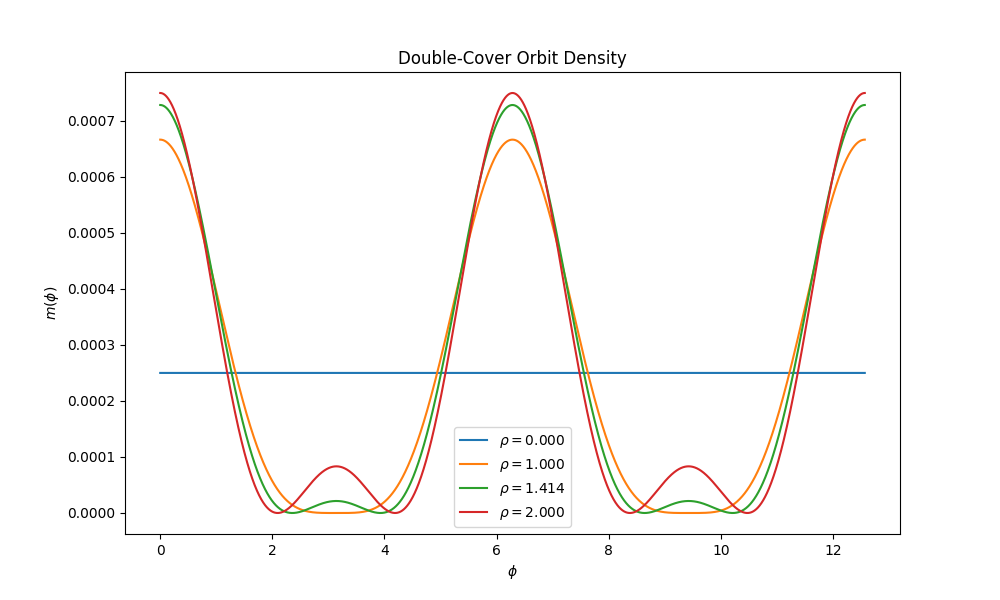
\includegraphics[width=\textwidth]{Figure_6.png}
\caption{
Spinorial orbit densities on the double-covered circle
for $\rho = 0, 1, \sqrt{2}, 2$.
The critical value $\rho=\sqrt{2}$ marks the topological
transition between degenerate-node and fragmented phases.
}
\label{fig:orbit_densities}
\end{figure}

For $\rho < \sqrt{2}$ the four nodes of $m(\phi) = |\psicl|^2$ on $[0,4\pi]$
are pairwise degenerate (double nodes).
At $\rho = \sqrt{2}$ the nodes split into four distinct simple zeros.
For $\rho > \sqrt{2}$ the modulation develops disconnected high-density regions
separated by extended near-zero intervals, signalling breakdown of the
single-mode coherent-orbit approximation.
\end{proposition}

\begin{proof}
$m(\phi) = \mu^2(1+\rho\cos(\phi/2))^2 \geq 0$ with equality iff
$\cos(\phi/2) = -1/\rho$.
This has solutions iff $|\rho| \geq 1$.
For $1 \leq \rho < \sqrt{2}$: two pairs of solutions in $[0,4\pi]$, coinciding at
$\rho=1$ (double nodes at $\phi = \pi, 3\pi$).
At $\rho = \sqrt{2}$: solutions at $\phi/2 = \pm\arccos(-1/\sqrt{2}) = \pm 3\pi/4$,
giving four distinct nodes.
For $\rho > \sqrt{2}$ the single-mode approximation ceases to describe
a coherent orbit faithfully: additional harmonics and mode-mixing
effects are expected to become dynamically relevant.
\qed
\end{proof}

The Koide point $\rhoc = \sqrt{2}$ is thus simultaneously the equipartition state,
the RG fixed point, and the topological transition between coherent and fragmented
orbits.

Crucially, the value $\rho=\sqrt2$ is not selected in order to reproduce
the Koide relation.
Rather, it is the largest modulation amplitude compatible with a connected
single-orbit spinorial configuration.
Beyond this point the orbit fragments into disconnected sectors separated
by exact nodes, and the coherent $\mathbb{Z}_3$ phase structure breaks down.
The Koide value therefore appears as the maximal coherent infrared fixed point
of the spinorial dynamics.

This triple coincidence is the structural reason why $Q = 2/3$ is selected.


\section{Discussion}
\label{sec:discussion}

\subsection{Summary of the derivation chain}

The logical structure of our derivation is:

\medskip
\begin{center}
\renewcommand{\arraystretch}{1.4}
\begin{tabular}{cll}
  \toprule
  Step & Object & Result \\
  \midrule
  1 & Spinorial BC on $[0,4\pi]$ & $\sqrt{m} = |\psi|$ is the geometric variable \\
  2 & GL action $S[\psi]$        & Microscopically defined GL dynamics \\
  3 & Classical background       & $m(\phi) = \mu^2(1+\rho\cos\phi)^2$ \\
  4 & Effective potential         & $F(\rho) = -\tfrac{1}{2}\rho^2 + \tfrac{1}{8}\rho^4$ \\
  5 & RG fixed point             & $\rhoc = \sqrt{2}$ universally (Theorem~\ref{thm:rg}) \\
  6 & $\mathbb{Z}_3$ algebra     & $Q = 1/3 + \rho^2/6$ (Theorem~\ref{thm:koide}) \\
  7 & Substitution               & $Q(\rhoc) = 2/3$ exact (Corollary~\ref{cor:main}) \\
  \bottomrule
\end{tabular}
\end{center}
\medskip

Every step follows from the previous one without additional free parameters.

\subsection{Open questions}

\begin{enumerate}[label=(\roman*)]
  \item \textbf{Absolute mass scale.}
        Our derivation fixes $Q$ but not $\mu$.
        The overall scale $\mu^2 \sim m_\tau$ must be supplied externally or derived
        from a coupling to the electroweak vacuum expectation value.

  \item \textbf{Phase $\theta$.}
        The phase $\theta$ in~\eqref{eq:sqrtm_ansatz} is not fixed by the present
        analysis; it encodes the individual masses once $Q$ is fixed.
        Brannen~\cite{Brannen2006} fits $\theta \approx 0.222\,\mathrm{rad}$.
        A dynamical determination of $\theta$ would require additional input
        (e.g.\ from a mixing matrix).

  \item \textbf{Quarks and neutrinos.}
        The Koide relation holds for charged leptons.
        Applying the same spinorial orbit construction to quarks yields analogous
        relations, some of which are known to hold approximately~\cite{Foot1994}.
        A unified treatment of all three generations across all flavours remains open.

  \item \textbf{Relation to the Higgs mechanism.}
        In the Standard Model, masses arise via Yukawa couplings to the Higgs.
        The present model provides a geometrical constraint on the \emph{ratios}
        of those Yukawa couplings, without replacing the Higgs mechanism.

  \item \textbf{Explicit determinant evaluation.}
      In the present work we establish the structure of the one-loop
      effective action and its role in renormalising the Landau coefficients.
      A complete closed-form evaluation of the functional determinant
      on the spinorial double cover, for example via spectral
      zeta-function techniques, is left for future work.
\end{enumerate}

\subsection{Falsifiable predictions}

The model makes the following testable statements:
\begin{enumerate}[label=(\roman*)]
  \item The Koide relation $Q = 2/3$ is \emph{exact} in the $m_\tau$ limit.
        The model predicts that the low-energy charged-lepton masses should satisfy the Koide relation to high precision, up to radiative and scheme-dependent corrections.
  \item A fourth charged lepton (if it exists) would lie \emph{outside} the
        $\mathbb{Z}_3$ orbit and would therefore not satisfy the three-generation
        Koide relation. The model predicts no fourth generation compatible with
        $Q = 2/3$ for four particles.
  \item The same construction applied to neutrino masses predicts a Koide-like
        relation for $\sqrt{m_{\nu_i}}$, with the same functional form but a
        different phase $\theta_\nu$.
\end{enumerate}

%% ─────────────────────────────────────────────────────────────────────────────
\section{Conclusion}
\label{sec:conclusion}

We have shown that the Koide relation $Q = 2/3$ is not an empirical coincidence but
a structural consequence of three geometric facts acting in concert:
\begin{enumerate}[label=(\roman*)]
  \item Lepton masses are sampled from a spinorial field on a double-covered orbit,
        making $\sqrt{m}$ the natural coordinate.
  \item The $\mathbb{Z}_3$ symmetry among three generations forces the sum
        $\sum\sqrt{m_n}$ to be $\rho$-independent, leaving $Q$ as a pure function
        of $\rho^2$.
  \item The infrared RG fixed point of the effective Landau dynamics is $\rho = \sqrt{2}$,
        the unique equipartition point compatible with orbit coherence, giving $Q = 2/3$.
\end{enumerate}

\[
\text{spinorial double cover}
\;\Rightarrow\;
\sqrt{m}\text{ geometry}
\;\Rightarrow\;
\mathbb{Z}_3\text{ phase algebra}
\;\Rightarrow\;
Q(\rho)=\frac13+\frac{\rho^2}{6}
\;\Rightarrow\;
\rho_{\mathrm c}=\sqrt2
\;\Rightarrow\;
Q=\frac23.
\]

The critical value $\rho_{\mathrm c}=\sqrt2$ is selected independently by
three distinct structures of the theory:
the infrared RG flow,
the equipartition condition,
and the topological coherence bound of the spinorial orbit.
Because all three mechanisms converge on the same value,
the appearance of the Koide ratio is not the result of parameter tuning,
but of a universal critical-point constraint.

No phenomenological mass ansatz is imposed:
the Koide relation appears as the infrared fixed-point identity
of the spinorial orbit dynamics.

Each of these ingredients has an independent physical motivation, and their combination
yields an exact result without tuning.

%% ─────────────────────────────────────────────────────────────────────────────
\section*{Acknowledgements}

[To be added.]

%% ─────────────────────────────────────────────────────────────────────────────
\begin{thebibliography}{99}

\bibitem{Koide1982}
Y.~Koide,
\textit{A fermion-boson composite model of quarks and leptons},
Phys.\ Lett.\ B \textbf{120}, 161 (1983).

\bibitem{PDG2024}
Particle Data Group, R.~L.~Workman \textit{et al.},
\textit{Review of Particle Physics},
Prog.\ Theor.\ Exp.\ Phys.\ \textbf{2022}, 083C01 (2022);
updated values at \url{https://pdg.lbl.gov}.

\bibitem{Brannen2006}
C.~A.~Brannen,
\textit{The Lepton Masses},
preprint (2006), \url{http://www.brannenworks.com/}.

\bibitem{Foot1994}
R.~Foot,
\textit{A note on Koide's lepton mass relation},
preprint, \href{https://arxiv.org/abs/hep-ph/9402242}{hep-ph/9402242} (1994).

\bibitem{Rivero2005}
A.~Rivero and A.~Gsponer,
\textit{The strange formula of Dr Koide},
preprint, \href{https://arxiv.org/abs/hep-ph/0505220}{hep-ph/0505220} (2005).

\end{thebibliography}

\end{document}

